% Generated by thesis/ch7/exp1/c4_case_figures.py -- do not edit by hand.
\begin{figure}[tbp]
  \centering
  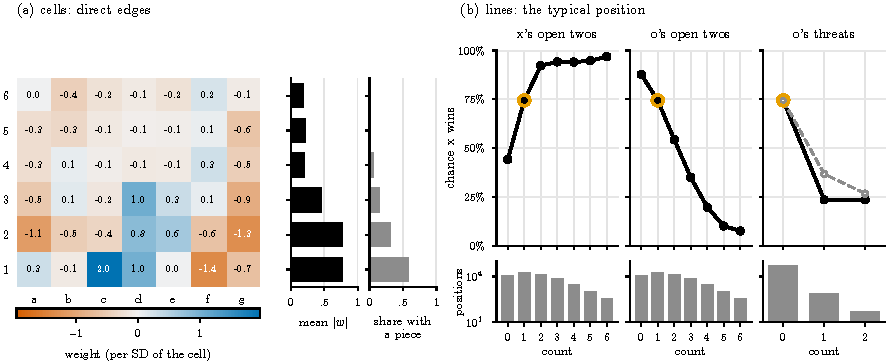
\includegraphics[width=\textwidth,height=0.8\textheight,keepaspectratio]{figures/ch7/c4-case-contrast.pdf}
  \caption{Connect-4: the cells network's direct edges and the lines network's response. (a) Cells network: the weight of each cell's direct edge to the output (blue raises the chance that x wins, red lowers it; row 1 is the bottom of the board); bars: per row, the mean absolute weight (black) and the share of training positions with a piece on a cell of the row (grey). (b) Lines network: the predicted chance that x wins as one line feature changes, all others at the typical position (orange circle); o's threats: solid, every threat on an even row; dashed, the threat count alone, its row parity left at zero. Grey bars: training positions at each count (log scale).}
  \label{fig:ch7-c4-case-contrast}
\end{figure}
